\documentclass[10pt,fleqn, openany, landscape, twocolumn]{book} % Default font size and left-justified equations

%%%%%%%%%%%%%%%%%%%%%%%%%%%%%%%%%%%%%%%%%
% The Legrand Orange Book
% Structural Definitions File
% Version 2.1 (26/09/2018)
%
% Original author:
% Mathias Legrand (legrand.mathias@gmail.com) with modifications by:
% Vel (vel@latextemplates.com)
% 
% This file was downloaded from:
% http://www.LaTeXTemplates.com
%
% License:
% CC BY-NC-SA 3.0 (http://creativecommons.org/licenses/by-nc-sa/3.0/)
%
%%%%%%%%%%%%%%%%%%%%%%%%%%%%%%%%%%%%%%%%%

%----------------------------------------------------------------------------------------
%	VARIOUS REQUIRED PACKAGES AND CONFIGURATIONS
%----------------------------------------------------------------------------------------

\usepackage[table]{xcolor}

\usepackage{graphicx}
\usepackage{tabularx} % Required for including pictures
\usepackage{pgf,tikz,tkz-tab,eurosym,yhmath, stmaryrd}
\usepackage{pgfplots}
\usepackage{mathrsfs}
\usetikzlibrary{patterns}
\usetikzlibrary{trees}
\graphicspath{{../../Pictures/}}
\usepackage{multicol} 


\usepackage[english]{babel} % English language/hyphenation
\usepackage{icomma}
\usepackage{enumitem} % Customize lists
\setlist{nolistsep, nosep, nolistsep} % Reduce spacing between bullet points and numbered lists

\usepackage{booktabs} % Required for nicer horizontal rules in tables

 % Required for specifying colors by name


\definecolor{ocre}{RGB}{243,102,25} % Define the orange color used for highlighting throughout the book

\usepackage{listings}

\definecolor{codegreen}{rgb}{0,0.6,0}
\definecolor{codegray}{rgb}{0.5,0.5,0.5}
\definecolor{codepurple}{rgb}{0.58,0,0.82}
\definecolor{backcolour}{rgb}{0.95,0.95,0.92}

\lstdefinestyle{mystyle}{
    backgroundcolor=\color{backcolour},   
    commentstyle=\color{codegreen},
    keywordstyle=\color{magenta},
    numberstyle=\tiny\color{codegray},
    stringstyle=\color{codepurple},
    basicstyle=\ttfamily\footnotesize,
    breakatwhitespace=false,         
    breaklines=true,                 
    captionpos=b,                    
    keepspaces=true,                 
    numbers=left,                    
    numbersep=5pt,                  
    showspaces=false,                
    showstringspaces=false,
    showtabs=false,                  
    tabsize=2
}

\lstset{style=mystyle}

%----------------------------------------------------------------------------------------
% Paramétrage XSIM
%----------------------------------------------------------------------------------------

\usepackage[no-files]{xsim}


\DeclareExerciseEnvironmentTemplate{myex}{%
    \textbf{%
      \hypertarget{ex:\ExerciseID}{\sffamily{\ensuremath{\blacktriangleright}} Exercice \GetExerciseProperty{counter} \GetExerciseProperty{subtitle} --}
      \hyperlink{sol:\ExerciseID}{Voir le corrigé}%
    }\par
}{\par\smallskip}

\DeclareExerciseEnvironmentTemplate{mysol}{%
    \textbf{%
      \hypertarget{sol:\ExerciseID}{\sffamily{\ensuremath{\blacktriangleright}} Correction \GetExerciseProperty{counter} --}
      \hyperlink{ex:\ExerciseID}{Voir l'énoncé}%
    }\par
}{\par\medskip}

\xsimsetup{
  exercise/template = myex ,
  solution/template = mysol 
}

%Collection exercices

\DeclareExerciseTagging{topic}

\xsimsetup{collect}

%----------------------------------------------------------------------------------------
% SYMBOLES
%----------------------------------------------------------------------------------------

\newcommand\imCMsym[4][\mathord]{%
  \DeclareFontFamily{U} {#2}{}
  \DeclareFontShape{U}{#2}{m}{n}{
    <-6> #25
    <6-7> #26
    <7-8> #27
    <8-9> #28
    <9-10> #29
    <10-12> #210
    <12-> #212}{}
  \DeclareSymbolFont{CM#2} {U} {#2}{m}{n}
  \DeclareMathSymbol{#4}{#1}{CM#2}{#3}
}
\newcommand\alsoimCMsym[4][\mathord]{\DeclareMathSymbol{#4}{#1}{CM#2}{#3}}

\imCMsym{cmmi}{124}{\CMjmath}

\newcommand{\Oij}{(O\,;\,\vec{\imath}\,,\, \vec{\CMjmath} )}
\newcommand{\Oijk}{(O\,;\,\vec{\imath}\,,\, \vec{\CMjmath}\,,\,\vec{k})}

\newcommand\e{\mathrm{e}}
\newcommand\R{\mathbb{R}}
\newcommand\N{\mathbb{N}}


%----------------------------------------------------------------------------------------
%	MARGINS
%----------------------------------------------------------------------------------------

\usepackage{geometry} % Required for adjusting page dimensions and margins

\geometry{
	paper=a4paper, % Paper size, change to letterpaper for US letter size
	top=3cm, % Top margin
	bottom=3cm, % Bottom margin
	left=2cm, % Left margin
	right=2cm, % Right margin
	headheight=14pt, % Header height
	footskip=1.4cm, % Space from the bottom margin to the baseline of the footer
	headsep=10pt, % Space from the top margin to the baseline of the header
	%showframe, % Uncomment to show how the type block is set on the page
}

\setlength{\parindent}{0pt}
\parskip=5pt



%----------------------------------------------------------------------------------------
%	FONTS
%----------------------------------------------------------------------------------------

\usepackage{avant} % Use the Avantgarde font for headings
\usepackage{times} % Use the Times font for headings
\usepackage{mathptmx} % Use the Adobe Times Roman as the default text font together with math symbols from the Sym­bol, Chancery and Com­puter Modern fonts

%\usepackage{microtype} % Slightly tweak font spacing for aesthetics
%\usepackage[utf8]{inputenc} % Required for including letters with accents
\usepackage[T1]{fontenc} % Use 8-bit encoding that has 256 glyphs

%----------------------------------------------------------------------------------------
%	BIBLIOGRAPHY AND INDEX
%----------------------------------------------------------------------------------------

\usepackage[style=numeric,citestyle=numeric,sorting=nyt,sortcites=true,autopunct=true,babel=hyphen,hyperref=true,abbreviate=false,backref=true,backend=biber]{biblatex}
\addbibresource{bibliography.bib} % BibTeX bibliography file
\defbibheading{bibempty}{}

\usepackage{calc} % For simpler calculation - used for spacing the index letter headings correctly
\usepackage{makeidx} % Required to make an index
\makeindex % Tells LaTeX to create the files required for indexing

%----------------------------------------------------------------------------------------
%	MAIN TABLE OF CONTENTS
%----------------------------------------------------------------------------------------

\usepackage{titletoc} % Required for manipulating the table of contents

\contentsmargin{0cm} % Removes the default margin

% Part text styling (this is mostly taken care of in the PART HEADINGS section of this file)
\titlecontents{part}
	[0cm] % Left indentation
	{\addvspace{20pt}\bfseries} % Spacing and font options for parts
	{}
	{}
	{}

% Chapter text styling
\titlecontents{chapter}
	[1.25cm] % Left indentation
	{\addvspace{12pt}\large\sffamily\bfseries} % Spacing and font options for chapters
	{\color{ocre!60}\contentslabel[\Large\thecontentslabel]{1.25cm}\color{ocre}} % Formatting of numbered sections of this type
	{\color{ocre}} % Formatting of numberless sections of this type
	{\color{ocre!60}\normalsize\;\titlerule*[.5pc]{.}\;\thecontentspage} % Formatting of the filler to the right of the heading and the page number

% Section text styling
\titlecontents{section}
	[1.25cm] % Left indentation
	{\addvspace{3pt}\sffamily\bfseries} % Spacing and font options for sections
	{\contentslabel[\thecontentslabel]{1.25cm}} % Formatting of numbered sections of this type
	{} % Formatting of numberless sections of this type
	{\hfill\color{black}\thecontentspage} % Formatting of the filler to the right of the heading and the page number

% Subsection text styling
\titlecontents{subsection}
	[1.25cm] % Left indentation
	{\addvspace{1pt}\sffamily\small} % Spacing and font options for subsections
	{\contentslabel[\thecontentslabel]{1.25cm}} % Formatting of numbered sections of this type
	{} % Formatting of numberless sections of this type
	{\ \titlerule*[.5pc]{.}\;\thecontentspage} % Formatting of the filler to the right of the heading and the page number

% Figure text styling
\titlecontents{figure}
	[1.25cm] % Left indentation
	{\addvspace{1pt}\sffamily\small} % Spacing and font options for figures
	{\thecontentslabel\hspace*{1em}} % Formatting of numbered sections of this type
	{} % Formatting of numberless sections of this type
	{\ \titlerule*[.5pc]{.}\;\thecontentspage} % Formatting of the filler to the right of the heading and the page number

% Table text styling
\titlecontents{table}
	[1.25cm] % Left indentation
	{\addvspace{1pt}\sffamily\small} % Spacing and font options for tables
	{\thecontentslabel\hspace*{1em}} % Formatting of numbered sections of this type
	{} % Formatting of numberless sections of this type
	{\ \titlerule*[.5pc]{.}\;\thecontentspage} % Formatting of the filler to the right of the heading and the page number

%----------------------------------------------------------------------------------------
%	MINI TABLE OF CONTENTS IN PART HEADS
%----------------------------------------------------------------------------------------

% Chapter text styling
\titlecontents{lchapter}
	[0em] % Left indentation
	{\addvspace{15pt}\large\sffamily\bfseries} % Spacing and font options for chapters
	{\color{ocre}\contentslabel[\Large\thecontentslabel]{1.25cm}\color{ocre}} % Chapter number
	{}  
	{\color{ocre}\normalsize\sffamily\bfseries\;\titlerule*[.5pc]{.}\;\thecontentspage} % Page number

% Section text styling
\titlecontents{lsection}
	[0em] % Left indentation
	{\sffamily\small} % Spacing and font options for sections
	{\contentslabel[\thecontentslabel]{1.25cm}} % Section number
	{}
	{}

% Subsection text styling (note these aren't shown by default, display them by searchings this file for tocdepth and reading the commented text)
\titlecontents{lsubsection}
	[.5em] % Left indentation
	{\sffamily\footnotesize} % Spacing and font options for subsections
	{\contentslabel[\thecontentslabel]{1.25cm}}
	{}
	{}

%----------------------------------------------------------------------------------------
%	HEADERS AND FOOTERS
%----------------------------------------------------------------------------------------


\usepackage{fancyhdr} % Required for header and footer configuration

\pagestyle{fancy}
\renewcommand{\chaptermark}[1]{\markboth{\sffamily\normalsize\bfseries\ \thechapter.\ #1}{}} % Chapter text font settings
\renewcommand{\sectionmark}[1]{\markright{\sffamily\normalsize\thesection\hspace{5pt}#1}{}} % Section text font settings
\fancyhf{} \fancyhead[LE,RO]{\sffamily\normalsize\thepage} % Font setting for the page number in the header
\fancyhead[LO]{\rightmark} % Print the nearest section name on the left side of odd pages
\fancyhead[RE]{\leftmark} % Print the current chapter name on the right side of even pages

\fancyfoot[L]{Jason LAPEYRONNIE}
\fancyfoot[R]{\href{http://mathoutils.fr}{http://mathoutils.fr}} % Uncomment to include a footer

\renewcommand{\headrulewidth}{0.5pt} % Thickness of the rule under the header
\renewcommand{\footrulewidth}{0.5pt} % Thickness of the rule under the header

\fancypagestyle{plain}{% Style for when a plain pagestyle is specified
	\fancyhead{}\renewcommand{\headrulewidth}{0pt}%
}

% Removes the header from odd empty pages at the end of chapters
\makeatletter
\renewcommand{\cleardoublepage}{
\clearpage\ifodd\c@page\else
\hbox{}
\vspace*{\fill}
\thispagestyle{empty}
\newpage
\fi}

%----------------------------------------------------------------------------------------
%	THEOREM STYLES
%----------------------------------------------------------------------------------------

\usepackage{amsmath,amsfonts,amssymb,amsthm} % For math equations, theorems, symbols, etc

\newcommand{\intoo}[2]{\mathopen{]}#1\,;#2\mathclose{[}}
\newcommand{\ud}{\mathop{\mathrm{{}d}}\mathopen{}}
\newcommand{\intff}[2]{\mathopen{[}#1\,;#2\mathclose{]}}
\renewcommand{\qedsymbol}{$\blacksquare$}
\newtheorem{notation}{Notation}[section]

% Boxed/framed environments
\newtheoremstyle{ocrenumbox}% Theorem style name
{0pt}% Space above
{0pt}% Space below
{\normalfont}% Body font
{}% Indent amount
{\small\bf\sffamily\color{ocre}}% Theorem head font
{\;:\;}% Punctuation after theorem head
{0.25em}% Space after theorem head
{\small\sffamily\color{ocre}\thmname{#1}\nobreakspace\thmnumber{\@ifnotempty{#1}{}\@upn{#2}}% Theorem text (e.g. Theorem 2.1)
\thmnote{\nobreakspace\the\thm@notefont\sffamily\bfseries\color{black}---\nobreakspace#3}} % Optional theorem note

\newtheoremstyle{blacknumex}% Theorem style name
{5pt}% Space above
{10pt}% Space below
{\normalfont}% Body font
{} % Indent amount
{\small\bf\sffamily}% Theorem head font
{\;:\;}% Punctuation after theorem head
{0.25em}% Space after theorem head
{\small\sffamily{\tiny\ensuremath{\blacksquare}}\nobreakspace\thmname{#1}\nobreakspace\thmnumber{\@ifnotempty{#1}{}\@upn{#2}}% Theorem text (e.g. Theorem 2.1)
\thmnote{\nobreakspace\the\thm@notefont\sffamily\bfseries---\nobreakspace#3}}% Optional theorem note

\newtheoremstyle{blacknumexo}% Theorem style name
{15pt}% Space above
{10pt}% Space below
{\normalfont}% Body font
{} % Indent amount
{\small\bf\sffamily}% Theorem head font
{}% Punctuation after theorem head
{0.5em}% Space after theorem head
{\small\sffamily{\ensuremath{\blacktriangleright}}\nobreakspace\thmname{#1}\nobreakspace\thmnumber{\@ifnotempty{#1}{}\@upn{#2}}% Theorem text (e.g. Theorem 2.1)
\thmnote{\nobreakspace\the\thm@notefont\sffamily\bfseries---\nobreakspace#3} \\}% Optional theorem note



\newtheoremstyle{blacknumbox} % Theorem style name
{0pt}% Space above
{5pt}% Space below
{}% Body font
{}% Indent amount
{\large\bf\sffamily}% Theorem head font
{\;:\;}% Punctuation after theorem head
{0.25em}% Space after theorem head
{\small\sffamily\thmname{#1}\nobreakspace\thmnumber{\@ifnotempty{#1}{}\@upn{#2}}% Theorem text (e.g. Theorem 2.1)
\thmnote{\nobreakspace\the\thm@notefont\sffamily\bfseries---\nobreakspace#3}}% Optional theorem note

% Non-boxed/non-framed environments
\newtheoremstyle{ocrenum}% Theorem style name
{5pt}% Space above
{5pt}% Space below
{\normalfont}% Body font
{}% Indent amount
{\small\bf\sffamily\color{ocre}}% Theorem head font
{\;:\;}% Punctuation after theorem head
{0.25em}% Space after theorem head
{\small\sffamily\color{ocre}\thmname{#1}\nobreakspace\thmnumber{\@ifnotempty{#1}{}\@upn{#2}}% Theorem text (e.g. Theorem 2.1)
\thmnote{\nobreakspace\the\thm@notefont\sffamily\bfseries\color{black}---\nobreakspace#3}} % Optional theorem note
\makeatother

% Defines the theorem text style for each type of theorem to one of the three styles above
\newcounter{dummy} 
\newcounter{thm}
\newcounter{correction}
\newcounter{qst}
\theoremstyle{ocrenumbox}
\newtheorem{theoremeT}[dummy]{Théorème}
\newtheorem{exerciseT}{Propriété}
\newtheorem{principeT}{Principe}
\theoremstyle{blacknumex}
\newtheorem{exampleT}{Exemple}
\theoremstyle{blacknumexo}
\newtheorem{exo}[thm]{Exercice}
\newtheorem{corr}[correction]{Correction}
\newtheorem{quest}[qst]{Question}
\theoremstyle{blacknumbox}
\newtheorem{vocabulary}{Vocabulary}[section]
\newtheorem{definitionT}{Définition}
\newtheorem{corollaryT}[dummy]{Corollary}
\theoremstyle{ocrenum}
\newtheorem{proofT}[dummy]{Démonstration}


%----------------------------------------------------------------------------------------
%	DEFINITION OF COLORED BOXES
%----------------------------------------------------------------------------------------

\RequirePackage[framemethod=default]{mdframed} % Required for creating the theorem, definition, exercise and corollary boxes

% Theorem box
\newmdenv[skipabove=7pt,
skipbelow=7pt,
backgroundcolor=black!5,
linecolor=ocre,
innerleftmargin=5pt,
innerrightmargin=5pt,
innertopmargin=10pt,
leftmargin=0cm,
rightmargin=0cm,
innerbottommargin=5pt]{tBox}

%Proposition box	  
\newmdenv[skipabove=7pt,
skipbelow=7pt,
rightline=false,
leftline=true,
topline=false,
bottomline=false,
backgroundcolor=ocre!10,
linecolor=ocre,
innerleftmargin=5pt,
innerrightmargin=5pt,
innertopmargin=10pt,
innerbottommargin=3pt,
leftmargin=0cm,
rightmargin=0cm,
linewidth=4pt]{eBox}	

% Definition box
\newmdenv[skipabove=7pt,
backgroundcolor=ocre!4,
skipbelow=7pt,
rightline=false,
leftline=true,
topline=false,
bottomline=false,
linecolor=ocre,
innerleftmargin=5pt,
innerrightmargin=5pt,
innertopmargin=10pt,
leftmargin=0cm,
rightmargin=0cm,
linewidth=4pt,
innerbottommargin=5pt]{dBox}	

% Corollary box
\newmdenv[skipabove=7pt,
skipbelow=7pt,
rightline=false,
leftline=true,
topline=false,
bottomline=false,
linecolor=gray,
backgroundcolor=black!5,
innerleftmargin=5pt,
innerrightmargin=5pt,
innertopmargin=5pt,
leftmargin=0cm,
rightmargin=0cm,
linewidth=4pt,
innerbottommargin=5pt]{cBox}

\newmdenv[skipabove=7pt,
skipbelow=7pt,
backgroundcolor=black!5,
innerleftmargin=5pt,
topline=false,
bottomline=false,
rightline=false,
leftline=false,
innerrightmargin=5pt,
innertopmargin=5pt,
leftmargin=0cm,
rightmargin=0cm,
innerbottommargin=5pt]{xBox}

% Creates an environment for each type of theorem and assigns it a theorem text style from the "Theorem Styles" section above and a colored box from above
\newenvironment{theorem}{\begin{tBox}\begin{theoremeT}}{\end{theoremeT}\end{tBox}}

\newenvironment{exo2}{\noindent \begin{exo}\item\relax \noindent \begin{eBox}\item\relax}{\end{eBox}\end{exo}}


\newenvironment{proposition}{\begin{eBox}\begin{exerciseT}}{\hfill{\color{ocre}}\end{exerciseT}\end{eBox}}		

\newenvironment{principe}{\begin{eBox}\begin{principeT}}{\hfill{\color{ocre}}\end{principeT}\end{eBox}}	
		  
\newenvironment{definition}{\begin{dBox}\begin{definitionT}}{\end{definitionT}\end{dBox}}	

\newenvironment{example}{\begin{xBox}\begin{exampleT}}{\hfill{\tiny\ensuremath{\blacksquare}}\end{exampleT}\end{xBox}}

\newenvironment{demonstration}{\begin{proofT}}{\hfill{\tiny\ensuremath{\square}}\end{proofT}}		
\newenvironment{corollary}{\begin{cBox}\begin{corollaryT}}{\end{corollaryT}\end{cBox}}	

%----------------------------------------------------------------------------------------
%	REMARK ENVIRONMENT
%----------------------------------------------------------------------------------------

\newenvironment{remark}{\par\vspace{5pt}\small % Vertical white space above the remark and smaller font size
\begin{list}{}{
\leftmargin=25pt % Indentation on the left
\rightmargin=15pt}\item\ignorespaces % Indentation on the right
\makebox[-2.5pt]{
\begin{tikzpicture}[overlay]
\node[draw=ocre!60,line width=1pt,circle,fill=ocre!25,font=\sffamily\bfseries,inner sep=2pt,outer sep=0pt] at (-15pt,0pt){\textcolor{ocre}{R}};\end{tikzpicture}} % Orange R in a circle
\advance\baselineskip -1pt}{\end{list}\vskip5pt} % Tighter line spacing and white space after remark

%----------------------------------------------------------------------------------------
%	SECTION NUMBERING IN THE MARGIN
%----------------------------------------------------------------------------------------

\makeatletter
\renewcommand{\@seccntformat}[1]{\llap{\textcolor{ocre}{\csname the#1\endcsname}\hspace{1em}}}                    
\renewcommand{\section}{\@startsection{section}{1}{\z@}
{-4ex \@plus -1ex \@minus -.4ex}
{1ex \@plus.2ex }
{\normalfont\LARGE\sffamily\bfseries}}
\renewcommand{\subsection}{\@startsection {subsection}{2}{\z@}
{-3ex \@plus -0.1ex \@minus -.4ex}
{0.5ex \@plus.2ex }
{\normalfont\sffamily\bfseries}}
\renewcommand{\subsubsection}{\@startsection {subsubsection}{3}{\z@}
{-2ex \@plus -0.1ex \@minus -.2ex}
{.2ex \@plus.2ex }
{\normalfont\small\sffamily\bfseries}}                        
\renewcommand\paragraph{\@startsection{paragraph}{4}{\z@}
{-2ex \@plus-.2ex \@minus .2ex}
{.1ex}
{\normalfont\small\sffamily\bfseries}}

%----------------------------------------------------------------------------------------
%	PART HEADINGS
%----------------------------------------------------------------------------------------

% Numbered part in the table of contents
\newcommand{\@mypartnumtocformat}[2]{%
	\setlength\fboxsep{0pt}%
	\noindent\colorbox{ocre!20}{\strut\parbox[c][.7cm]{\ecart}{\color{ocre!70}\Large\sffamily\bfseries\centering#1}}\hskip\esp\colorbox{ocre!40}{\strut\parbox[c][.7cm]{\linewidth-\ecart-\esp}{\Large\sffamily\centering#2}}%
}

% Unnumbered part in the table of contents
\newcommand{\@myparttocformat}[1]{%
	\setlength\fboxsep{0pt}%
	\noindent\colorbox{ocre!40}{\strut\parbox[c][.7cm]{\linewidth}{\Large\sffamily\centering#1}}%
}

\newlength\esp
\setlength\esp{4pt}
\newlength\ecart
\setlength\ecart{1.2cm-\esp}
\newcommand{\thepartimage}{}%
\newcommand{\partimage}[1]{\renewcommand{\thepartimage}{#1}}%
\def\@part[#1]#2{%
\ifnum \c@secnumdepth >-2\relax%
\refstepcounter{part}%
\addcontentsline{toc}{part}{\texorpdfstring{\protect\@mypartnumtocformat{\thepart}{#1}}{\partname~\thepart\ ---\ #1}}
\else%
\addcontentsline{toc}{part}{\texorpdfstring{\protect\@myparttocformat{#1}}{#1}}%
\fi%
\startcontents%
\markboth{}{}%
{\thispagestyle{empty}%
\begin{tikzpicture}[remember picture,overlay]%
\node at (current page.north west){\begin{tikzpicture}[remember picture,overlay]%	
\fill[ocre!20](0cm,0cm) rectangle (\paperwidth,-\paperheight);
\node[anchor=north] at (4cm,-3.25cm){\color{ocre!40}\fontsize{220}{100}\sffamily\bfseries\thepart}; 
\node[anchor=south east] at (\paperwidth-1cm,-\paperheight+1cm){\parbox[t][][t]{8.5cm}{
\printcontents{l}{0}{\setcounter{tocdepth}{1}}% The depth to which the Part mini table of contents displays headings; 0 for chapters only, 1 for chapters and sections and 2 for chapters, sections and subsections
}};
\node[anchor=north east] at (\paperwidth-1.5cm,-3.25cm){\parbox[t][][t]{15cm}{\strut\raggedleft\color{white}\fontsize{30}{30}\sffamily\bfseries#2}};
\end{tikzpicture}};
\end{tikzpicture}}%
\@endpart}
\def\@spart#1{%
\startcontents%
\phantomsection
{\thispagestyle{empty}%
\begin{tikzpicture}[remember picture,overlay]%
\node at (current page.north west){\begin{tikzpicture}[remember picture,overlay]%	
\fill[ocre!20](0cm,0cm) rectangle (\paperwidth,-\paperheight);
\node[anchor=north east] at (\paperwidth-1.5cm,-3.25cm){\parbox[t][][t]{15cm}{\strut\raggedleft\color{white}\fontsize{30}{30}\sffamily\bfseries#1}};
\end{tikzpicture}};
\end{tikzpicture}}
\addcontentsline{toc}{part}{\texorpdfstring{%
\setlength\fboxsep{0pt}%
\noindent\protect\colorbox{ocre!40}{\strut\protect\parbox[c][.7cm]{\linewidth}{\Large\sffamily\protect\centering #1\quad\mbox{}}}}{#1}}%
\@endpart}
\def\@endpart{\vfil\newpage
\if@twoside
\if@openright
\null
\thispagestyle{empty}%
\newpage
\fi
\fi
\if@tempswa
\twocolumn
\fi}

%----------------------------------------------------------------------------------------
%	CHAPTER HEADINGS
%----------------------------------------------------------------------------------------

% A switch to conditionally include a picture, implemented by Christian Hupfer
\newif\ifusechapterimage
\usechapterimagetrue
\newcommand{\thechapterimage}{}%
\newcommand{\chapterimage}[1]{\ifusechapterimage\renewcommand{\thechapterimage}{#1}\fi}%
\newcommand{\autodot}{.}
\def\@makechapterhead#1{%
{\parindent \z@ \raggedright \normalfont
\ifnum \c@secnumdepth >\m@ne
\if@mainmatter
\begin{tikzpicture}[remember picture,overlay]
\node at (current page.north west)
{\begin{tikzpicture}[remember picture,overlay]
\node[anchor=north west,inner sep=0pt] at (0,0) {\ifusechapterimage\includegraphics[width=\paperwidth]{\thechapterimage}\fi};
\draw[anchor=west] (\Gm@lmargin,-3cm) node [line width=2pt,rounded corners=15pt,draw=ocre,fill=white,fill opacity=0.5,inner sep=15pt]{\strut\makebox[22cm]{}};
\draw[anchor=west] (\Gm@lmargin+.3cm,-3cm) node {\huge\sffamily\bfseries\color{black}\thechapter\autodot~#1\strut};
\end{tikzpicture}};
\end{tikzpicture}
\else
\begin{tikzpicture}[remember picture,overlay]
\node at (current page.north west)
{\begin{tikzpicture}[remember picture,overlay]
\node[anchor=north west,inner sep=0pt] at (0,0) {\ifusechapterimage\includegraphics[width=\paperwidth]{\thechapterimage}\fi};
\draw[anchor=west] (\Gm@lmargin,-3cm) node [line width=2pt,rounded corners=15pt,draw=ocre,fill=white,fill opacity=0.5,inner sep=15pt]{\strut\makebox[22cm]{}};
\draw[anchor=west] (\Gm@lmargin+.3cm,-3cm) node {\huge\sffamily\bfseries\color{black}#1\strut};
\end{tikzpicture}};
\end{tikzpicture}
\fi\fi\par\vspace*{50\p@}}}

%-------------------------------------------

\def\@makeschapterhead#1{%
\begin{tikzpicture}[remember picture,overlay]
\node at (current page.north west)
{\begin{tikzpicture}[remember picture,overlay]
\node[anchor=north west,inner sep=0pt] at (0,0) {\ifusechapterimage\includegraphics[width=\paperwidth]{\thechapterimage}\fi};
\draw[anchor=west] (\Gm@lmargin,-3cm) node [line width=2pt,rounded corners=15pt,draw=ocre,fill=white,fill opacity=0.5,inner sep=15pt]{\strut\makebox[22cm]{}};
\draw[anchor=west] (\Gm@lmargin+.3cm,-3cm) node {\huge\sffamily\bfseries\color{black}#1\strut};
\end{tikzpicture}};
\end{tikzpicture}
\par\vspace*{50\p@}}
\makeatother

%----------------------------------------------------------------------------------------
%	LINKS
%----------------------------------------------------------------------------------------

\usepackage{hyperref}
\hypersetup{hidelinks,backref=true,pagebackref=true,hyperindex=true,colorlinks=false,breaklinks=true,urlcolor=ocre,bookmarks=true,bookmarksopen=false}

\usepackage{bookmark}
\bookmarksetup{
open,
numbered,
addtohook={%
\ifnum\bookmarkget{level}=0 % chapter
\bookmarksetup{bold}%
\fi
\ifnum\bookmarkget{level}=-1 % part
\bookmarksetup{color=ocre,bold}%
\fi
}
}

\renewcommand*\thesection{\arabic{section}}

\newcommand*{\coord}[3]{% 
  \ensuremath{\overrightarrow{#1}\, 
    \begin{pmatrix} 
      #2\\ 
      #3 
    \end{pmatrix}}}
    
  \newcommand*{\coordb}[2]{% 
  \ensuremath{ 
    \begin{pmatrix} 
      #1\\ 
      #2 
    \end{pmatrix}}}

\newcommand*{\coorde}[4]{% 
  \renewcommand{\arraystretch}{1}\ensuremath{\overrightarrow{#1}\, 
    \begin{pmatrix} 
      #2\\ 
      #3 \\
      #4
    \end{pmatrix}}}    
  \newcommand*{\coordbe}[3]{% 
 \renewcommand{\arraystretch}{1} \ensuremath{ 
    \begin{pmatrix} 
      #1\\ 
      #2 \\
      #3
    \end{pmatrix}}}  
    
\newcommand{\Card}{\mathrm{Card}}

\usepackage{soul}
\begin{document}

\chapterimage{../../Pictures/background}

\subsection*{Fonctions et limites de référence}

%x^2
\fbox{\begin{minipage}{0.48\linewidth}


\hl{$x\mapsto x^n$, avec $n$ pair}

\begin{minipage}{0.5\linewidth}

$\displaystyle\lim_{x \to -\infty}x^n=+\infty$ 

$\displaystyle\lim_{x \to +\infty}x^n=+\infty$ 


\end{minipage}
\begin{minipage}{0.2\linewidth}
\begin{center}
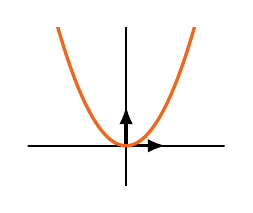
\begin{tikzpicture}[scale=0.5]
\clip (-2.5,-1) rectangle (2.5,3);
\draw [thick] (-4,0)--(7,0);
\draw [thick] (0,-4) -- (0,5);
\draw [very thick,->,>=latex] (0,0)--(0,1);
\draw [very thick,->,>=latex] (0,0)--(1,0);
\draw [very thick, ocre,domain=-3:3,samples=100] plot (\x,{\x*\x});
\end{tikzpicture}
\end{center}
\end{minipage}
\end{minipage}}
\hfill
%x^3
\fbox{\begin{minipage}{0.48\linewidth}


\hl{$x\mapsto x^n$, avec $n$ impair}

\begin{minipage}{0.5\linewidth}

$\displaystyle\lim_{x \to -\infty}x^n=-\infty$ 

$\displaystyle\lim_{x \to +\infty}x^n=+\infty$ 


\end{minipage}
\begin{minipage}{0.2\linewidth}
\begin{center}
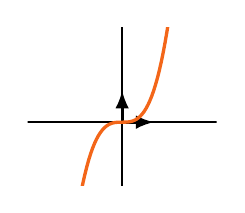
\begin{tikzpicture}[scale=0.4]
\clip (-3,-2) rectangle (3,3.);
\draw [thick] (-4,0)--(7,0);
\draw [thick] (0,-4) -- (0,5);
\draw [very thick,->,>=latex] (0,0)--(0,1);
\draw [very thick,->,>=latex] (0,0)--(1,0);
\draw [very thick, ocre,domain=-3:3,samples=100] plot (\x,{\x*\x*\x});
\end{tikzpicture}
\end{center}
\end{minipage}
\end{minipage}}


\fbox{\begin{minipage}{0.48\linewidth}


\hl{$x\mapsto e^x$}

\begin{minipage}{0.5\linewidth}

$\displaystyle\lim_{x \to -\infty}e^x=0$ 

$\displaystyle\lim_{x \to +\infty}e^x=+\infty$ 


\end{minipage}
\begin{minipage}{0.2\linewidth}
\begin{center}
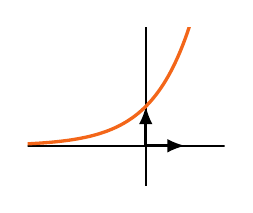
\begin{tikzpicture}[scale=0.5]
\clip (-3,-1) rectangle (2,3);
\draw [thick] (-4,0)--(7,0);
\draw [thick] (0,-4) -- (0,5);
\draw [very thick,->,>=latex] (0,0)--(0,1);
\draw [very thick,->,>=latex] (0,0)--(1,0);
\draw [very thick, ocre,domain=-3:3,samples=100] plot (\x,{exp(\x)});
\end{tikzpicture}
\end{center}
\end{minipage}
\end{minipage}}
\hfill
\fbox{\begin{minipage}{0.48\linewidth}


\hl{$x\mapsto \ln(x)$}

\begin{minipage}{0.5\linewidth}

$\displaystyle\lim_{x \to 0}\ln(x)=-\infty$ 

$\displaystyle\lim_{x \to +\infty}\ln(x)=+\infty$ 


\end{minipage}
\begin{minipage}{0.2\linewidth}
\begin{center}
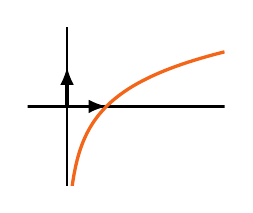
\begin{tikzpicture}[scale=0.5]
\clip (-1,-2) rectangle (4,2);
\draw [thick] (-4,0)--(7,0);
\draw [thick] (0,-4) -- (0,5);
\draw [very thick,->,>=latex] (0,0)--(0,1);
\draw [very thick,->,>=latex] (0,0)--(1,0);
\draw [very thick, ocre,domain=0.1:4,samples=100] plot (\x,{ln(\x)});
\end{tikzpicture}
\end{center}
\end{minipage}
\end{minipage}}


\fbox{\begin{minipage}{0.48\linewidth}


\hl{$x\mapsto \sqrt{x}$}

\begin{minipage}{0.5\linewidth}

$\displaystyle\lim_{x \to +\infty}\sqrt{x}=+\infty$ 

\textbf{Non dérivable en 0}

\end{minipage}
\begin{minipage}{0.2\linewidth}
\begin{center}
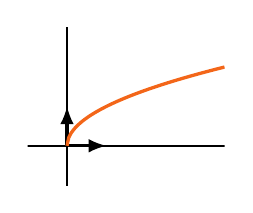
\begin{tikzpicture}[scale=0.5]
\clip (-1,-1) rectangle (4,3);
\draw [thick] (-4,0)--(7,0);
\draw [thick] (0,-4) -- (0,5);
\draw [very thick,->,>=latex] (0,0)--(0,1);
\draw [very thick,->,>=latex] (0,0)--(1,0);
\draw [very thick, ocre,domain=0:4,samples=100] plot (\x,{sqrt(\x)});
\end{tikzpicture}
\end{center}
\end{minipage}
\end{minipage}}
\hfill
\fbox{\begin{minipage}{0.48\linewidth}


\begin{minipage}{0.7\linewidth}
\hl{$x\mapsto \frac{1}{x}$}

$\displaystyle\lim_{x \to -\infty}\frac{1}{x}=0^-$,  $\displaystyle\lim_{x \to +\infty}\frac{1}{x}=0^+$

$\displaystyle\lim_{x \to 0^+}\frac{1}{x}=+\infty$, $\displaystyle\lim_{x \to 0^-}\frac{1}{x}=-\infty$


\end{minipage}
\begin{minipage}{0.2\linewidth}
\begin{center}
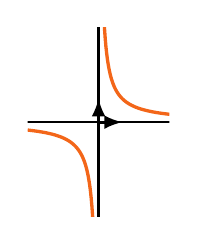
\begin{tikzpicture}[scale=0.3]
\clip (-3,-4) rectangle (3,4);
\draw [thick] (-4,0)--(7,0);
\draw [thick] (0,-4) -- (0,5);
\draw [very thick,->,>=latex] (0,0)--(0,1);
\draw [very thick,->,>=latex] (0,0)--(1,0);
\draw [very thick, ocre,domain=-3:-0.01,samples=100] plot (\x,1/\x);
\draw [very thick, ocre,domain=0.01:3,samples=100] plot (\x,1/\x);
\end{tikzpicture}
\end{center}
\end{minipage}
\end{minipage}}


\fbox{\begin{minipage}{0.48\linewidth}
$x\mapsto \cos(x)$
\begin{center}
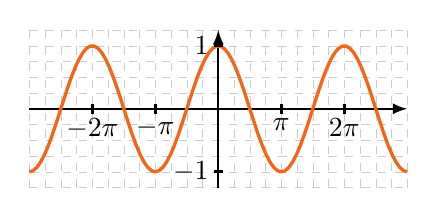
\begin{tikzpicture}[scale=0.2]
\draw [dashed, very thin, gray!40] (-12,-5) grid (12,5);
\draw [>=latex,->,thick] (-12,0) -- (12,0);
\draw [>=latex,->,thick] (0,-5) -- (0,5);
\draw [ocre, very thick,samples=100,domain=-12:12] plot (\x, {4*cos(pi*\x/4 r)}); 
\draw [very thick] (4,-0.3) -- (4,0.3);
\draw [very thick] (8,-0.3) -- (8,0.3);
\draw [very thick] (-4,-0.3) -- (-4,0.3);
\draw [very thick] (-8,-0.3) -- (-8,0.3);
\draw [very thick] (0.3,4) -- (-0.3,4);
\draw [very thick] (0.3,-4) -- (-0.3,-4);
\draw (4,0) node[below] {$\pi$};
\draw (-4,0) node[below] {$-\pi$};
\draw (8,0) node[below] {$2\pi$};
\draw (-8,0) node[below] {$-2\pi$};
\draw (0,4) node[left] {$1$};
\draw (0,-4) node[left] {$-1$};
\end{tikzpicture}
\end{center}\end{minipage}}\hfill
\fbox{\begin{minipage}{0.48\linewidth}

$x\mapsto \sin(x)$
\begin{center}
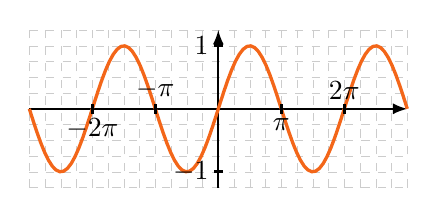
\begin{tikzpicture}[scale=0.2]
\draw [dashed, very thin, gray!40] (-12,-5) grid (12,5);
\draw [>=latex,->,thick] (-12,0) -- (12,0);
\draw [>=latex,->,thick] (0,-5) -- (0,5);
\draw [ocre, very thick,samples=100,domain=-12:12] plot (\x, {4*sin(pi*\x/4 r)}); 
\draw [very thick] (4,-0.3) -- (4,0.3);
\draw [very thick] (8,-0.3) -- (8,0.3);
\draw [very thick] (-4,-0.3) -- (-4,0.3);
\draw [very thick] (-8,-0.3) -- (-8,0.3);
\draw [very thick] (0.3,4) -- (-0.3,4);
\draw [very thick] (0.3,-4) -- (-0.3,-4);
\draw (4,0) node[below ] {$\pi$};
\draw (-4,0) node[above] {$-\pi$};
\draw (8,0) node[above] {$2\pi$};
\draw (-8,0) node[below] {$-2\pi$};
\draw (0,4) node[left] {$1$};
\draw (0,-4) node[left] {$-1$};
\end{tikzpicture}
\end{center}\end{minipage}}

\hl{\textbf{Asymptotes}} :
\begin{itemize}
\item Si $\displaystyle\lim_{x \to \pm \infty}f(x)=a$, la droite d'équation $y=a$ est asymptote à la courbe de $f$ en $\pm \infty$.
\item Si $\displaystyle\lim_{x \to b}f(x)=\pm \infty$ ($b$ fini), la droite d'équation $x=b$ est asymptote à la courbe de $f$.
\end{itemize}

\hl{\textbf{Suites géométriques}} : Si $q>1$, alors $\displaystyle\lim_{n\to +\infty}q^n=+\infty$. Si $-1<q<1$, alors $\displaystyle\lim_{n\to + \infty}q^n=0$.




\subsection*{Opérations sur les limites (suites ou fonctions)}


\begin{tabularx}{\linewidth}{|l|X|X|X|X|X|X|}
\hline
$\displaystyle \lim_{x \to a} f(x)$ & $l_1$ & $l_1$ & $l_1$ & $+\infty$ & $-\infty$ & $+\infty$\\
\hline
$\displaystyle \lim_{x \to a} g(x)$ & $l_2$ & $+\infty$ & $-\infty$ & $+\infty$ & $-\infty$ & $-\infty$\\
\hline
$\displaystyle \lim_{x \to a} (f+g)(x)$ & $l_1+l_2$ & $+\infty$ & $-\infty$ & $+\infty$ & $-\infty$ & \textbf{F.I.} \\
\hline
\end{tabularx}

\begin{tabularx}{\linewidth}{|l|X|X|X|X|}
\hline
$\displaystyle \lim_{x \to a} f(x)$ & $l_1 $ & $l_1 \neq 0$ &  $\infty$ & $0$ \\
\hline
$\displaystyle \lim_{x \to a} g(x)$ & $l_2$ & $\infty$  & $\infty$  & $\infty$ \\
\hline
$\displaystyle \lim_{x \to a} (fg)(x)$ & $l_1\,l_2$ & $\infty$ (r.s.)  & $\infty$ (r.s.) & \textbf{F.I.} \\
\hline
\end{tabularx}


\begin{tabularx}{\linewidth}{|l|X|X|X|X|c|c|}
\hline
$\displaystyle \lim_{x \to a} f(x)$ & $l_1 $ & $l_1$ & $l_1 \neq 0$ & $\infty$  & $0$ & $\infty$\\
\hline
$\displaystyle \lim_{x \to a} g(x)$ & $l_2 \neq 0$ & $\infty$ &  $0^+$ ou $0^-$ &  $l_2$, $0^+$ ou $0^-$ & $0$ & $\infty$ \\
\hline
$\displaystyle \lim_{x \to a} \left(\dfrac{f}{g}\right)(x)$ & $\dfrac{l_1}{l_2}$ & 0 & $\infty$  (r.s.)  & $\infty$ (r.s.) & \multicolumn{2}{|c|}{\textbf{F.I.}} \\
\hline\end{tabularx}

\textbf{Méthodes pour lever une indéterminée} :
\begin{itemize}
\item Factorisation par le termes de plus haut degré
\item Quantité conjuguée (différence de racines carrées)
\item Utilisation des croissances comparées
\end{itemize}


\hl{\textbf{Croissances comparées}} : Pour tout entier naturel non nul $n$,

\begin{tabularx}{\linewidth}{XXXX}
$\displaystyle\lim_{x\to + \infty}\dfrac{e^x}{x^n}=+\infty$ & $\displaystyle\lim_{x\to - \infty}x^ne^x=0$ & $\displaystyle\lim_{x\to + \infty}\dfrac{\ln(x)}{x^n}=0$ & $\displaystyle\lim_{x\to 0^+} x^n \ln(x)=0$
\end{tabularx}

\hl{\textbf{Compositions de limites}}

Si $\displaystyle\lim_{x\to a}f(x)=b$ et $\displaystyle\lim_{x\to b}g(x)=c$ alors $\displaystyle\lim_{x \to a}(g\circ f)(x)=c$

\subsection*{Théorèmes sur les limites}

\hl{\textbf{Théorème de comparaison}} : Soit $a$ un réel ou $\pm \infty$. Soit $f$ et $g$ deux fonctions définies sur un intervalle $I$ dont $a$ est un élément ou un bord.
\begin{itemize}
\item Si, pour tout $x\in I$, $f(x)\geqslant g(x)$ et $\displaystyle \lim_{x \to a} g(x)=+\infty$, alors $\displaystyle \lim_{x \to a} f(x)=+\infty$
\item Si, pour tout $x\in I$, $f(x)\leqslant g(x)$ et $\displaystyle \lim_{x \to a} g(x)=-\infty$, alors $\displaystyle \lim_{x \to a} f(x)=-\infty$
\end{itemize}

\hl{\textbf{Théorème d'encadrement :}} Soit $a$ un réel. Soit $f$, $g$ et $h$ trois fonctions définies sur un intervalle $I$ dont $a$ est un élément ou un bord.

Si, pour tout $x\in I$, $f(x)\leqslant g(x)\leqslant h(x)$ et si $f$ et $h$ admettent une même limite \textbf{finie} $\ell$ en $a$, alors $g$ admet également une limite finie en $a$ et $\displaystyle \lim_{x \to +\infty} g(x)=\ell$.

\hl{\textbf{Suites monotones}} : 
\begin{itemize}
\item Si $(u_n)$ est \textbf{croissante et majorée} par $M$, alors $(u_n)$ converge et $\displaystyle\lim_{n \to +\infty}u_n\leqslant M$.
\item Si $(u_n)$ est \textbf{décroissante et minorée} par $m$, alors $(u_n)$ converge et $\displaystyle\lim_{n \to +\infty}u_n\geqslant m$.
\end{itemize}
\textbf{Il est en revanche faux de dire que la limite vaut automatiquement le majorant ou le minorant en question ! }

\hl{\textbf{Algorithme de seuil}}\\
\begin{minipage}{0.45 \linewidth}
\begin{lstlisting}[language=python]
#Suite croissante
def seuil(s):
	u = #valeur de u(0)
	n = 0
	while u < s :
		u = #expression de u(n+1)
		n = n + 1
	return n
\end{lstlisting}
\end{minipage}\hfill\begin{minipage}{0.45 \linewidth}
\begin{lstlisting}[language=python]
#Suite decroissante
def seuil(s):
	u = #valeur de u(0)
	n = 0
	while u > s :
		u = #expression de u(n+1)
		n = n + 1
	return n
\end{lstlisting}
\end{minipage}

\hl{\textbf{Théorème du point fixe}} : Soit $f$ une fonction définie, \textbf{continue} et à valeurs dans un intervalle $I$ . Soit $(u_n)$ une suite telle que $u_0 \in I$ et pour tout entier naturel $n$, $u_{n+1}=f(u_n)$. \\ Si $(u_n)$ converge vers $\ell \in I$, alors $f(\ell)=\ell$.

%\textbf{Une fois que l'on a établi la convergence de la suite, déterminer sa limite revient à résoudre une équation.}

\subsection*{Théorème des valeurs intermédiaires}
\begin{minipage}{0.5\linewidth}
Soit $f$ une fonction \textbf{continue} sur $]a;b[$.\\ Alors pour tout réel $k$ compris entre $\displaystyle\lim_{x \to a}f(x)$ et $\displaystyle\lim_{x \to b}f(x)$, l'équation $f(x)=k$ admet au moins une solution sur $]a;b[$.
\vskip5pt
Si de plus, la fonction $f$ est \textbf{strictement monotone} sur $]a;b[$, alors une telle solution est unique.\end{minipage}\hfill\begin{minipage}{0.45\linewidth}
\begin{lstlisting}[language = python]
#Algorithme de dichotomie
#Resolution approchee de f(x)=0
def dicho(f, a, b, p):
	while abs(b-a) > 10 ** (-p):
		m = (a+b)/2
		if f(a) * f(m) < 0:
			b = m
		else :
			a = m
	return m
\end{lstlisting}
\end{minipage}

\subsection*{Propriétés de calcul}

\hl{\textbf{Second degré}} : Racines et signe de $ax^2+bx+c$. On pose $\Delta=b^2-4ac$.
\begin{itemize}
\item Si $\Delta >0$, $x_1=\frac{-b-\sqrt{\Delta}}{2a}$, $x_2=\frac{-b+\sqrt{\Delta}}{2a}$. Signe de $a$ à l'extérieur des racines.
\item Si $\Delta=0$, $x_0=-\frac{b}{2a}$. Signe de $a$ partout.
\item Si $\Delta<0$, pas de racine réelle, signe de $a$ partout.
\end{itemize}

\hl{\textbf{Avec l'exponentielle}} : Pour tout réel $x$, $e^x>0$. Soit $a$, $b$ des réels, $n$ un entier relatif

\begin{tabularx}{\linewidth}{XXXX}
$e^a\times e^b = a^{a+b}$ & $e^{-a}=\dfrac{1}{e^a}$ & $\dfrac{e^a}{e^b}=e^{a-b}$ & $(e^a)^n=e^{na}$
\end{tabularx}

\hl{\textbf{Avec le logarithme}} : Soit $x>0$, on a, $\ln(x)>0$ ssi $x>1$. Soit $a$, $b \in \mathbb{R}_+^*$, $n\in\mathbb{Z}$.

\begin{tabularx}{\linewidth}{XXX}
$\ln(ab)=\ln(a)+\ln(b)$ & $\ln\left(\dfrac{a}{b}\right)=\ln(a)-\ln(b)$ & $\ln(a^n)=n \times \ln(a)$
\end{tabularx}

\subsection*{Dérivées, primitives}
\renewcommand{\arraystretch}{2.2}
\begin{tabularx}{\linewidth}{|X|X|X|}

\hline
Fonction $f$ & Dérivée & \textbf{UNE} Primitive $F$  \\
\hline
$x \mapsto x^n$, $n\in \mathbb{N}^*$ & $x\mapsto nx^{n-1}$ & $x\mapsto \dfrac{x^{n+1}}{n+1}$   \\
\hline
$x \mapsto \dfrac{1}{x^n}$, $n\in \mathbb{N}^*$ & $x\mapsto -\dfrac{n}{x^{n+1}}$ & $x\mapsto -\dfrac{1}{(n-1)x^{n-1}}$, ($n \geqslant 2$) \\
\hline
$x\mapsto \sqrt{x}$ & $x \mapsto\dfrac{1}{2\sqrt{x}}$ & $\dfrac{2}{3}x\sqrt{x}$ (non exigible)  \\
\hline
$x \mapsto e^{ax+b}$ & $x\mapsto a \times e^{ax+b}$ & $x\mapsto \dfrac{e^{ax+b}}{a}$ \\
\hline
$x \mapsto \ln(x)$ & $x\mapsto \dfrac{1}{x}$ &  $x\mapsto x\ln(x)-x$ (non exigible)  \\
\hline
$x \mapsto \sin(x)$ & $x\mapsto \cos(x)$ &  $x\mapsto -\cos(x)$   \\
\hline
$x \mapsto \cos(x)$ & $x\mapsto -\sin(x)$ &  $x\mapsto \sin(x)$   \\
\hline
\end{tabularx}

\subsection*{Opérations sur les dérivées}
\begin{tabularx}{\linewidth}{XXX}
$(u+v)'=u'+v'$ & $(uv)'=u'v+uv'$  & $\left(\dfrac{u}{v}\right)'=\dfrac{u'v-uv'}{v^2}$\\
\end{tabularx}
\begin{tabularx}{\linewidth}{XXXX}
$\left(\dfrac{1}{u}\right)'=-\dfrac{u'}{u^2}$ & $(e^u)'=u' e^u$ & $(\ln(u))'=\dfrac{u'}{u}$& $(\sqrt{u})'=\dfrac{u'}{2\sqrt{u}}$\\ \end{tabularx}
\begin{tabularx}{\linewidth}{XXX}
 $(u^n)'=n\times u' \times u^{n-1}$& $(\cos(u))'=-u' \times \sin(u)$& $(\sin(u))'=u' \times \cos(u)$\end{tabularx}

\hl{\textbf{Équation de la tangente}} à la courbe de $f$ au point d'abscisse $a$ : $y=f'(a)(x-a)+f(a)$

\subsection*{Convexité, concavité}

\fbox{\begin{minipage}{0.65\linewidth}
\hl{Fonction convexe}
\begin{itemize}
\item En-dessous de ses cordes, au-dessus de ses tangentes
\item Dérivée croissante, dérivée seconde positive
\end{itemize}
\end{minipage}\hfill\begin{minipage}{0.3\linewidth}
\begin{center}
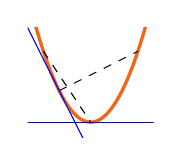
\begin{tikzpicture}[scale=0.2]
\clip (-2,-4) rectangle (6,3);

\draw [very thick, ocre,domain=-3:6,samples=100] plot (\x,{\x*\x/2-2*\x-1});
\draw [thin, dashed] (0,-1) -- (5,1.5);

\draw [thin, dashed] (-1,1.5) -- (2,-3);
\draw [thin, blue,domain=-3:6] plot (\x,-3);
\draw [thin, blue,domain=-3:6] plot (\x,-2*\x-1);
\end{tikzpicture}
\end{center}
\end{minipage}}

\fbox{\begin{minipage}{0.65\linewidth}
\hl{Fonction concave}
\begin{itemize}
\item Au-dessus de ses cordes, en-dessous de ses tangentes
\item Dérivée décroissante, dérivée seconde négative
\end{itemize}
\end{minipage}\hfill\begin{minipage}{0.3\linewidth}
\begin{center}
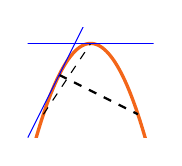
\begin{tikzpicture}[scale=0.2]
\clip (-2,-3) rectangle (6,4);
\draw [very thick, ocre,domain=-3:6,samples=100] plot (\x,{-(\x*\x/2-2*\x-1)});
\draw [thick, dashed] (0,1) -- (5,-1.5);

\draw [thin, dashed] (-1,-1.5) -- (2,3);
\draw [thin, blue,domain=-3:6] plot (\x,3);
\draw [thin, blue,domain=-3:6] plot (\x,2*\x+1);
\end{tikzpicture}
\end{center}
\end{minipage}}

\subsection*{Équations différentielles}

\hl{\textbf{Équation homogène}} $y'+ay=0$ : Solutions $x\mapsto Ce^{-ax}$, $C\in\mathbb{R}$

\hl{\textbf{Second membre constant}} $y'+ay=b$
\begin{itemize}
\item Recherche d'une solution constante $\varphi$ : on pose $y'=0$, on trouve $\varphi=\frac{b}{a}$
\item Solutions générale : $x\mapsto Ce^{-ax}+\frac{b}{a}$
\end{itemize}

\hl{\textbf{Second membre fonction}} $y'+ay=g$
\begin{itemize}
\item Recherche ou vérification d'une solution particulière $\varphi$
\item Solutions générale : $x\mapsto Ce^{-ax}+\varphi$
\end{itemize}

\textbf{Conditions initiales} : Une fois la solution générale trouvée, on remplace $x$ par $x_0$ et on résout une équation pour trouver $C$.

\subsection*{Calcul intégral}

\begin{minipage}{0.6\linewidth}
Définition de l'intégrale d'une fonction continue positive : \textbf{aire sous la courbe} exprimée en unité d'aire

Notation $\displaystyle\int_a^b f(x)dx$
\end{minipage}\hfill\begin{minipage}{0.35\linewidth}

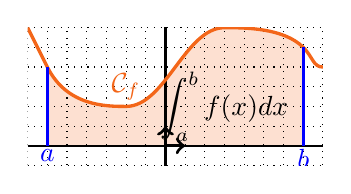
\begin{tikzpicture}[scale=0.25]
\clip (-7,-1) rectangle (8,6);

\filldraw [draw=black,fill=ocre!20]
(-6,4) .. controls (-5,2) and (-3,2) .. (-2,2)
.. controls (0,2) and (1,6) .. (3,6) .. controls (4,6) and (6,6) ..
(7,5) -- (7,0) -- (-6,0) -- cycle;

\draw [ thin, dotted] (-7,-3) grid (9,7);
\draw [thick] (-7,0)--(9,0);
\draw [thick] (0,-3)--(0,7);
\draw [->, very thick] (0,0)--(1,0);
\draw [->,very thick] (0,0)--(0,1);

\draw [ocre, very thick] (-7,6) .. controls (-6.5,5) and (-7,6).. (-6,4) .. controls (-5,2) and (-3,2) .. (-2,2)
.. controls (0,2) and (1,6) .. (3,6) .. controls (4,6) and (6,6) ..
(7,5) ..controls (7.5,4.5) and (7.5,4) .. (8,4);

\draw [blue, very thick] (7,0) -- (7,5);
\draw [blue, very thick] (-6,0) -- (-6,4);

\draw [ocre] (-2,3) node {$\mathcal{C}_f$};
\draw [blue] (-6,0.3) node[below] {$a$};
\draw [blue] (7,0.3) node[below] {$b$};
\draw (3,2) node {$\displaystyle\int_a^b f(x)dx$};
\end{tikzpicture}\end{minipage}

Si pour tout $x\in[a;b]$, $f(x)\leqslant g(x)$, l'aire entre les courbes de $f$ et $g$ vaut $\displaystyle\int_{a}^b(g-f)(x)dx$.

\hl{\textbf{Théorème fondamental}} : $F_a:x\mapsto \displaystyle\int_{a}^x f(t)dt$ est la primitive de $f$ qui s'annule en $a$.


\hl{\textbf{Calcul d'intégrale}} : Si $F$ est une primitive de $f$, $\displaystyle\int_a^bf(x)dx=[F(x)]^b_a=F(b)-F(a)$.

\hl{\textbf{Propriétés de l'intégrale}}\\
\begin{tabularx}{\linewidth}{Xl}
$\displaystyle\int_{a}^b (\lambda f+ \mu g)(t)dt=\lambda \displaystyle\int_{a}^b f(t)dt+ \mu\displaystyle\int_{a}^b g(t)dt\, ;$ & $\displaystyle\int_{a}^\textbf{\hl{c}} f(t)dt+\displaystyle\int_{\textbf{\hl{c}}}^b f(t)dt = \displaystyle\int_{a}^b f(t)dt$
\end{tabularx}

\hl{\textbf{Croissance}} : Si pour tout réel $x\in [a;b]$, on a $f(x)\leqslant g(x)$ alors $\displaystyle\int_{a}^b f(x)dx\leqslant \displaystyle\int_{a}^b g(x)dx$

\hl{\textbf{Valeur moyenne d'une fonction}} : \fbox{$m=\dfrac{1}{b-a}\displaystyle\int_{a}^b f(x)dx$}

\hl{\textbf{Intégration par parties (IPP)}} : \fbox{$\displaystyle\int_{a}^b (uv')(x)dx=[uv]_a^b-\displaystyle\int_{a}^b (u'v)(x)dx$}

\subsection*{Probabilités conditionnelles}

\hl{\textbf{Probabilité conditionnelle}} de $B$ sachant $A$ : $P_A(B)=\frac{P(A \cap B)}{P(A)}$

\hl{\textbf{Formule des probabilités totales}} :  On considère un événement $B$ et $A_1$, $A_2$, ..., $A_n$ un système complet d'événements de l'univers $\Omega$. Alors,
\[P(B)=P(B \cap A_1) + P(B \cap A_2) + \ldots + P(B \cap A_n) = \displaystyle\sum_{i=1}^{n} P(B\cap A_i)\]

\textbf{Indépendance} : Deux événements $A$ et $B$ sont indépendants si $P(A \cap B)=P(A)P(B)$.

\textbf{Arbre pondéré}
\vspace{-2.5cm}
\tikzstyle{level 1}=[level distance=6cm, sibling distance=4cm]
\tikzstyle{level 2}=[level distance=6cm, sibling distance=1.5cm]
\tikzstyle{level 3}=[level distance=10cm, sibling distance=0.3cm]

% Define styles for bags and leafs
\tikzstyle{bag} = [text centered]
\tikzstyle{part} = [circle]
\tikzstyle{end} = [circle, minimum width=3pt,fill, inner sep=0pt]
\begin{center}
\begin{tikzpicture}[scale=0.3,grow=right,sloped]
\node[bag] { }
    child {
        node[bag] {C} 
        child {
                node[bag] {F}
                edge from parent node[below] {$ $}
            }
        child {
               node[bag] {E}
               edge from parent node[above] {$ $}
            }
        child {
                node[bag] {D}
                edge from parent node[above] {$ $}
            }
            edge from parent node[above] {$ $} 
    }
    child {
        node[bag] {B}        
            child {
                node[bag] {F}
                edge from parent [black] node[below] {$ $}
            }
            child {
                node[bag] {E}
                edge from parent [black] node[above] {$ $}
            }
            child {
                node[bag] {D}
                edge from parent [black] node[above] {$ $}
            }
            edge from parent node[above] {$ $}
    }
     child {
        node[bag] {A}        
            child {
                node[bag] {F}
                edge from parent node[below] {$ $}
            }
            child {
                node[bag] {E}
                edge from parent node[above] {$ $}
            }
            child {
                node[bag] {D}
                child{
                	node[part] {$P(A\cap D) = P(A) \times P_A(D)$}
                	edge from parent [dashed,->]
                	}
                edge from parent node[above] {$P_A(D)$}
            }
            edge from parent node[above] {$P(A)$}
        };
\end{tikzpicture}
\end{center}
\vspace{-0.5cm}
\subsection*{Variable aléatoire}

\textbf{Définition} : Fonction définie sur un univers $\Omega$ à valeurs dans $\mathbb{R}$

\textbf{Loi d'une variable aléatoire réelle }: Fonction qui à tout réel $k$ associe $P(X=k)$.

\hl{\textbf{Espérance}} : Si $X$ prend les valeurs $x_1$, $x_2$, ..., $x_n$, \fbox{\[E(X)=x_1 \times P(X=x_1)+x_2 \times P(X=x_2) + \dots + x_n \times P(X=x_n)\]}
Interprétation : valeur moyenne de la variable aléatoire

\textbf{Linéarité de l'espérance} : $E(aX+b)=a \times E(X)+b$, $E(X+Y)=E(X)+E(Y)$

\hl{\textbf{Variance}} : $V(X)=E[(X-E(X))^2]=E[X^2]-E[X]^2$. Mesure de dispersion.

$V(aX+b)=a^2 \times V(X)$. Si $X$ et $Y$ sont \textbf{indépendantes}, $V(X+Y)=V(X)+V(Y)$.

\hl{\textbf{Écart-type}} : $\sigma(X)=\sqrt{V(X)}$

\subsection*{Dénombrement}

$\Card(A\cup B)= \Card(A) + \Card(B) - \Card(A \cap B)$, $\Card(A \times B)= \Card(A) \times \Card(B)$

\textbf{Factorielle} : $n! = n \times (n-1) \times \dots \times 3 \times 2 \times 1$, $0!=1$

Soit $A$ un ensemble de cardinal $n$
\begin{itemize}
\item \textbf{$p$-uplet} ou \textbf{$p$-liste} de $A$ : élément de $A^p$, il y en a $n^p$
\item \textbf{$p$-arrangement} de $A$ : $p$-uplet d'éléments distincts de $A$. Il y en a $\frac{n!}{(n-p)!}$
\item Cas $p=n$ : un $n$-arrangement de $A$ s'appelle une \textbf{permutation}.
\end{itemize}

\hl{\textbf{Coefficient binomial }}$\binom{n}{k}$ :  nombre de sous-ensembles de $A$ ayant $k$ éléments.

\begin{minipage}{0.5\linewidth}

\begin{tabularx}{\linewidth}{XX}
$\binom{n}{k}=\frac{n!}{k!(n-k)!}$, & $\binom{n}{k} = \binom{n}{n-k}$, \\ $\binom{n}{0}=\binom{n}{n} = 1$, & $\binom{n}{1}=\binom{n}{n-1}=n$.\end{tabularx}

\textbf{Relation de Pascal} : $\binom{n}{k} + \binom{n}{k+1} = \binom{n+1}{k+1}$. Permet de construire le triangle de Pascal.
\end{minipage}\hfill\begin{minipage}{0.45\linewidth}
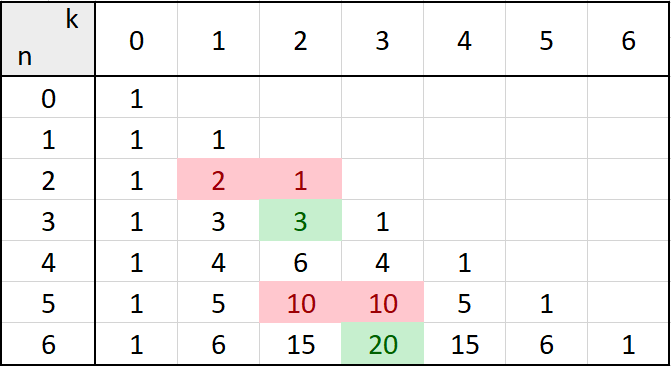
\includegraphics[scale=0.9]{pascal}\end{minipage}

\subsection*{Épreuve, loi, schéma de Bernoulli}

\hl{\textbf{Épreuve de Bernoulli}} : épreuve à deux issues, le succès $S$ et l'échec $\overline{S}$

\hl{\textbf{Loi de Bernoulli}} de paramètre $p$ : prend la valeur 1 avec proba $p$ et 0 avec proba $1-p$

\textbf{Schéma de Bernoulli} : Succession d'épreuves de Bernoulli identiques et indépendantes.

\subsection*{Loi binomiale}

\hl{\textbf{Loi binomiale}} de paramètres $n$ et $p$ : compte le nombre de succès d'un schéma de Bernoulli à $n$ épreuves, chaque épreuves ayant une probabilité de succès de $p$. $X\sim \mathcal{B}(n,p)$

\hl{\textbf{Formules}} Si $X$ suit une loi binomiale $\mathcal{B}(n,p)$, \fbox{$P(X=k)=\dbinom{n}{k}p^k(1-p)^{n-k}$}
\begin{tabularx}{\linewidth}{XXX}
$E(X)=np$ & $V(X)=np(1-p)$ & $\sigma(X)=\sqrt{np(1-p)}$\end{tabularx}
\vspace{-0.5cm}
\subsection*{Loi des grands nombres}

Soit $(X_1, X_2, \dots, X_n)$ un échantillon d'une v.a. réelle, $M_n=\frac{1}{n}(X_1+X_2+\dots+X_n)$
\begin{tabularx}{\linewidth}{XXX}
$E(M_n)=E(X_1)$ & $V(M_n)=\frac{V(X_1)}{n}$ & $\sigma(M_n)=\frac{\sigma(X_1)}{\sqrt{n}}$\end{tabularx}

\hl{\textbf{Inégalité de Bienaymé-Tchebychev}}: Pour tout $\delta > 0$, \fbox{$P(|X-E(X)| \geqslant \delta) \leqslant \frac{V(X)}{\delta ^2}$}

\hl{\textbf{Inégalité de concentration}} : Pour tout $\delta > 0$, \fbox{$P(|M_n-E(X_1)| \geqslant \delta) \leqslant \frac{V(X_1)}{n\delta ^2}$}

\subsection*{Géométrie dans l'espace}

\hl{\textbf{Colinéarité et applications}}

Deux vecteurs $\vec u$ et $\vec v$ sont \textbf{colinéaires} s'il existe un réel $k$ tel que $\vec u = k \vec v$ ou $\vec v = k \vec u$.

Droite passant par $A$ dirigée par $\vec u$ : ensemble des points $M$ tels que $\overrightarrow{AM}$ et $\vec u$ sont colinéaires.
\begin{itemize}
\item Deux droites sont \textbf{parallèles} ssi leurs vecteurs directeurs sont colinéaires.
\item Trois points $A$, $B$ et $C$ sont \textbf{alignés} si et seulement si $\overrightarrow{AB}$ et $\overrightarrow{AC}$ sont colinéaires.
\end{itemize}



\hl{\textbf{Coplanarité et applications}}

Trois vecteurs $\vec u$, $\vec v$ et $\vec w$ sont \textbf{coplanaires} si l'un de ces vecteurs peut s'exprimer comme combinaison linéaire des deux autres (par exemple $\vec u =\lambda \vec v + \mu \vec w$).

Plan passant par $A$ et dirigé par $\vec u$ et $\vec v$ non colinéaires : ensemble des points $M$ tels que $\overrightarrow{AM}$, $\vec u$ et $\vec v$ sont coplanaires.
\begin{itemize}
\item Quatre points $A$, $B$, $C$ et $D$ sont coplanaires s'il existe un plan passant par ces points
\item Quatre points $A$, $B$, $C$ et $D$ sont coplanaires ssi $\overrightarrow{AB}$, $\overrightarrow{AC}$ et $\overrightarrow{AD}$ sont coplanaires.
\item Deux droites sont coplanaires s'il existe un plan contenant ces deux droites
\end{itemize}

\hl{\textbf{Positions relatives}}

Pour deux droites :
\vspace{-1cm}
\tikzstyle{level 1}=[level distance=15cm, sibling distance=4cm]
\tikzstyle{level 2}=[level distance=15cm, sibling distance=2cm]
\tikzstyle{level 3}=[level distance=10cm, sibling distance=0.3cm]

% Define styles for bags and leafs
\tikzstyle{bag} = [text centered]
\tikzstyle{part} = [circle]
\tikzstyle{end} = [circle, minimum width=3pt,fill, inner sep=0pt]
\begin{center}
\begin{tikzpicture}[scale=0.3,grow=right,sloped]
\node[bag] { }
    child {
        node[bag] {Non coplanaires} 
    }
    child {
        node[bag] {Coplanaires}        
            child {
                node[bag] {Sécantes}
            }
            child {
                node[bag] {Parallèles}
            }
    };
\end{tikzpicture}
\end{center}

\begin{minipage}{0.23\linewidth}\begin{center}
\textbf{Droite sécante à un plan}
\end{center}
\begin{center}
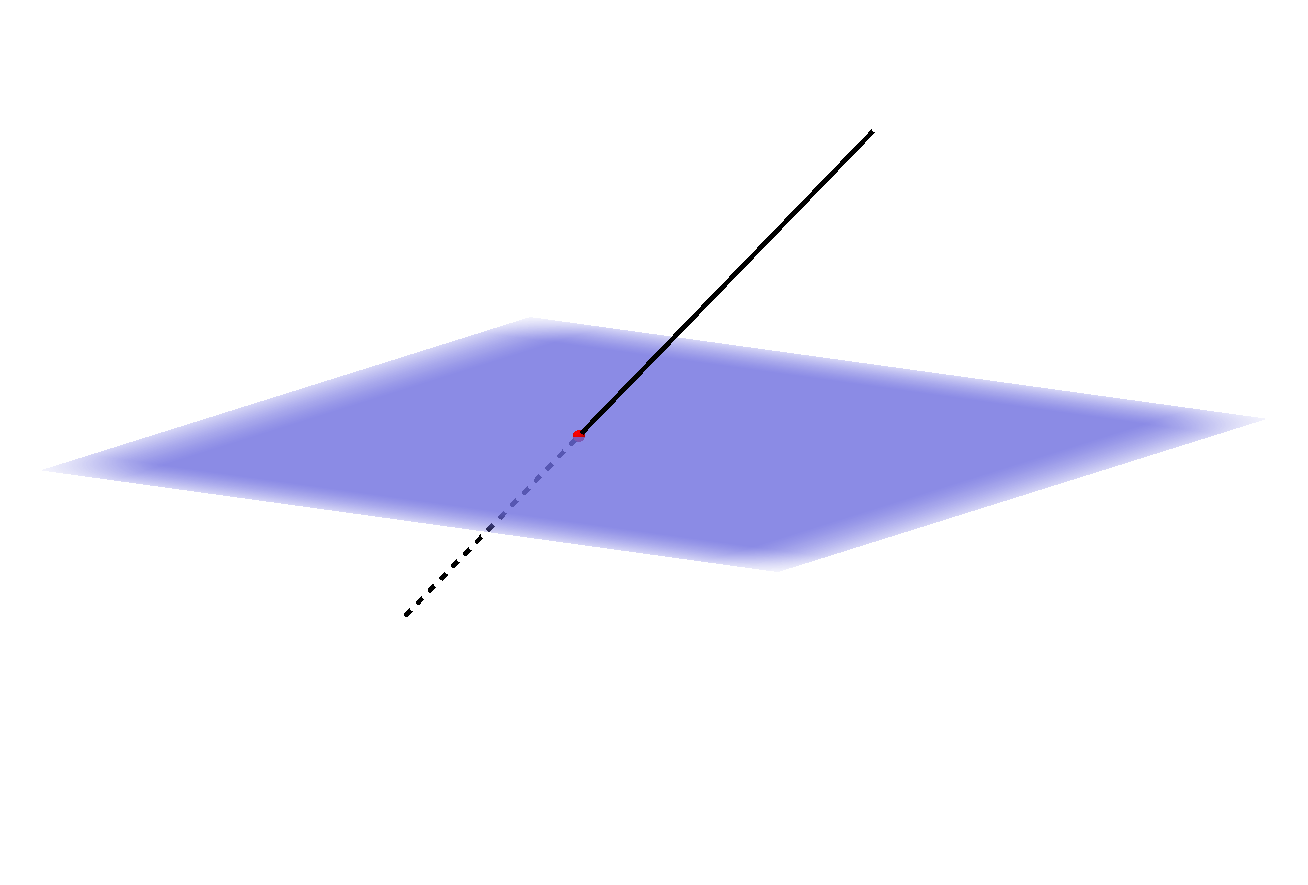
\includegraphics[width=0.8\linewidth]{relatif4}
\end{center}
\end{minipage}\hfill \begin{minipage}{0.23\linewidth}\begin{center}
\textbf{Droite parallèle à un plan}
\end{center}
\begin{center}
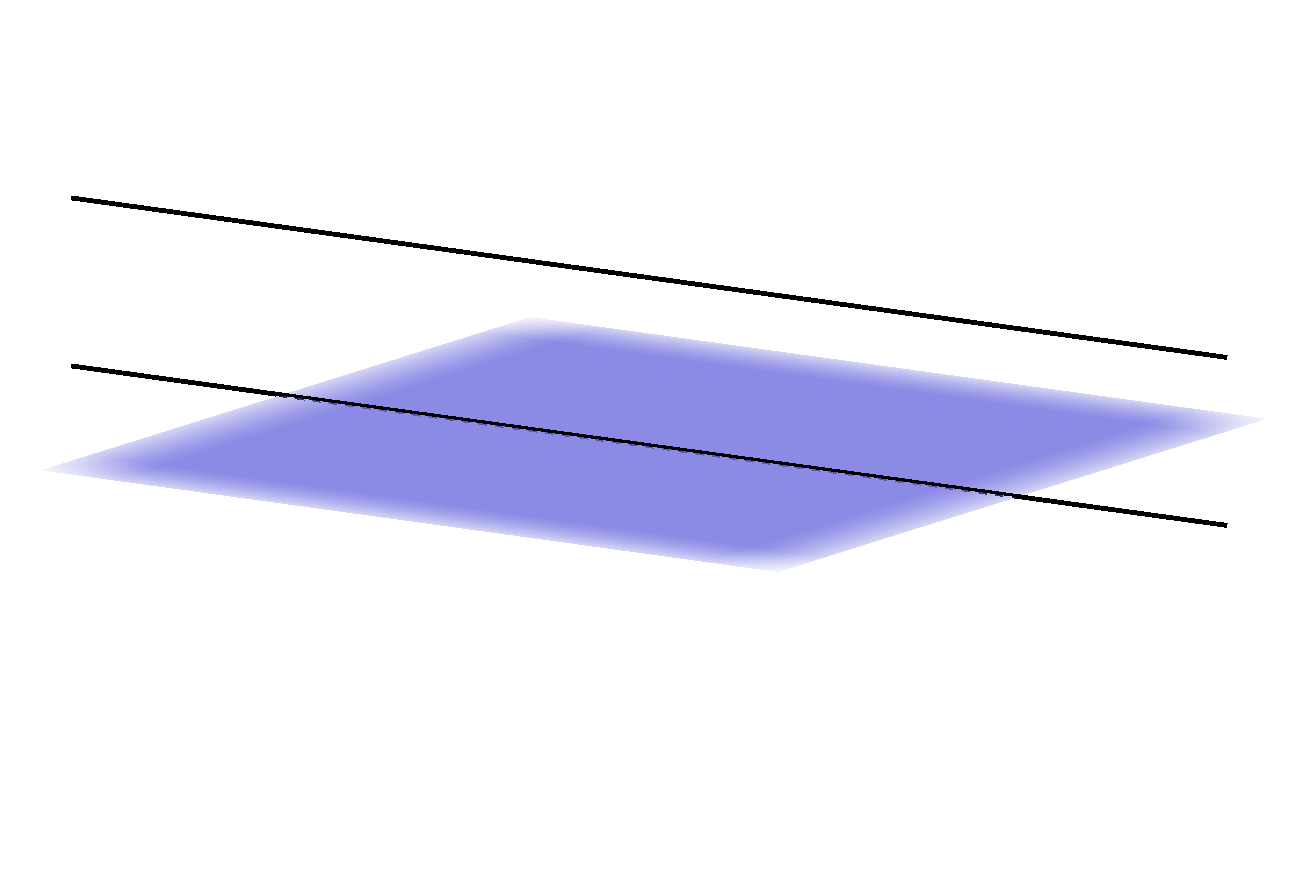
\includegraphics[width=0.8\linewidth]{relatif3}
\end{center}
\end{minipage}\hfill \begin{minipage}{0.23\linewidth}\begin{center}
\textbf{Plans sécants selon une droite}
\end{center}
\begin{center}
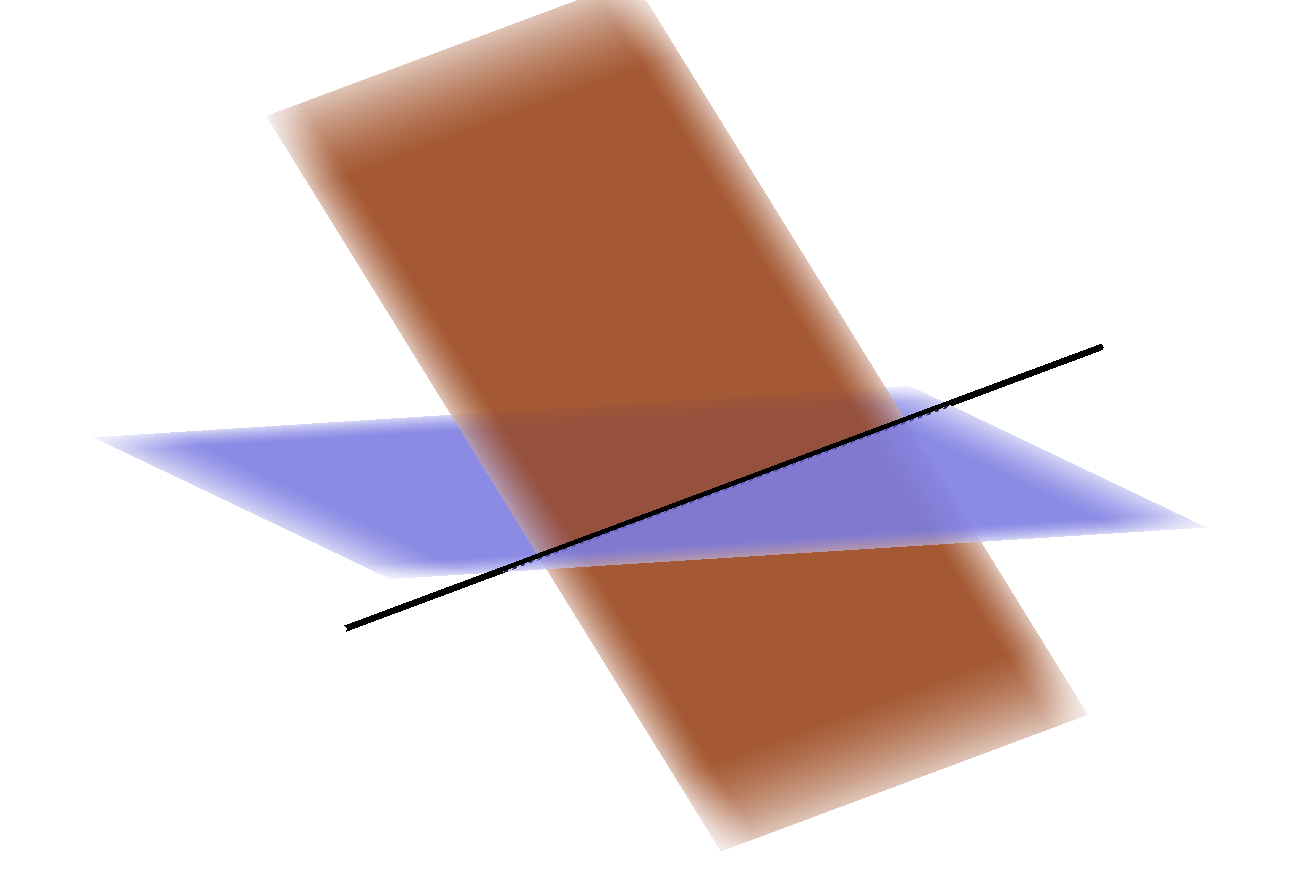
\includegraphics[width=0.7\linewidth]{relatif1}
\end{center}
\end{minipage}\hfill \begin{minipage}{0.23\linewidth}\begin{center}
\textbf{Plans parallèles}
\end{center}
\begin{center}
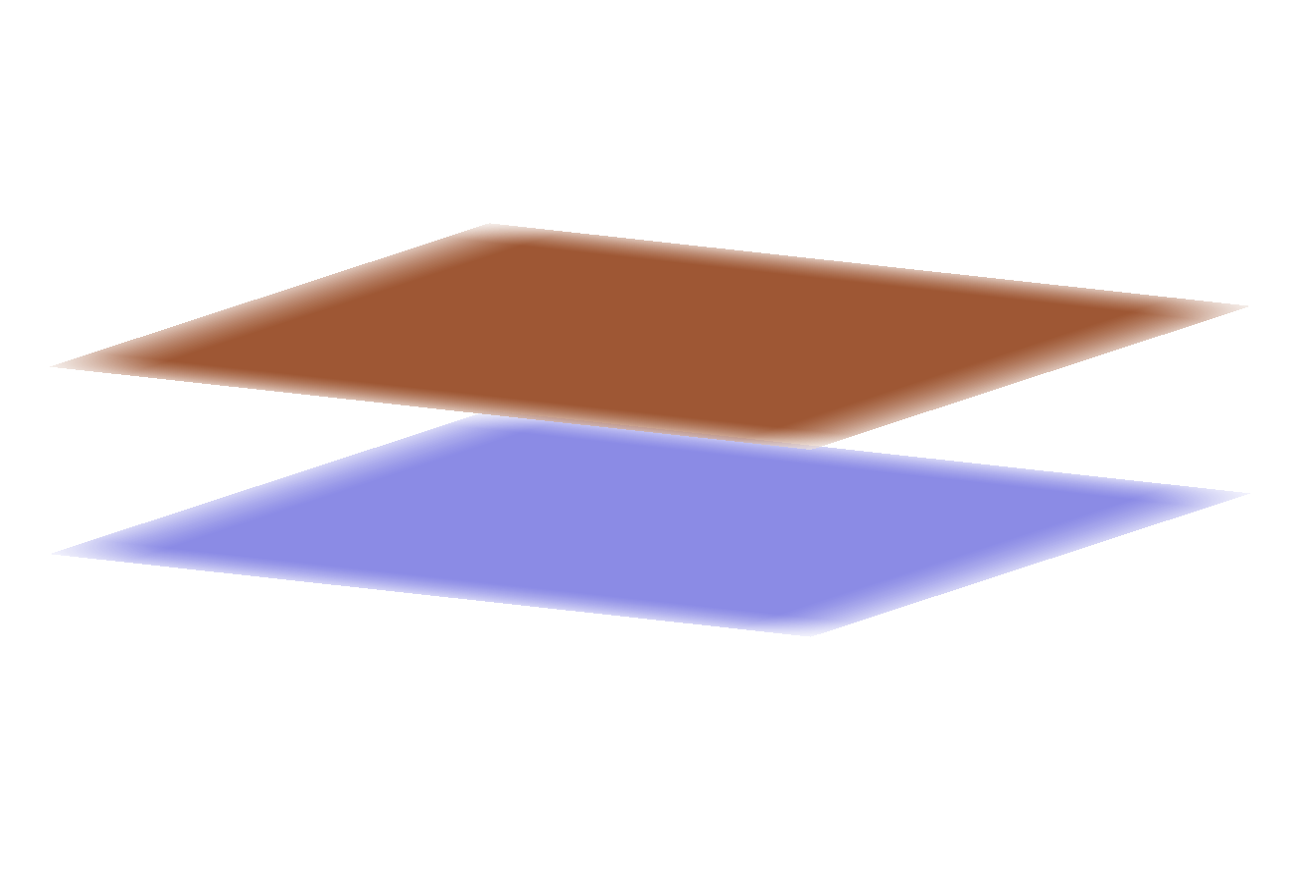
\includegraphics[width=0.7\linewidth]{relatif2}
\end{center}\end{minipage}

\hl{\textbf{Repérage dans l'espace}}

Un \textbf{repère} de l'espace est la donnée d'un point $O$ de l'espace et de trois vecteurs non coplanaires $\vec i$, $\vec j$, $\vec k$.
\renewcommand{\arraystretch}{1}
Pour tout vecteur $\vec u$, il existe des réels uniques $x$, $y$ et $z$ tq $\vec u=x\vec i + y \vec j + z \vec k$. 

On note $\vec u \begin{pmatrix}x\\y\\z\end{pmatrix}$. Si on a $A(x_A ; y_A ; z_A)$ et $B(x_B ; y_B ; z_B)$, alors $\overrightarrow{AB}\begin{pmatrix}x_B-x_A\\y_B-y_A\\z_B-z_A\end{pmatrix}$

Si $\renewcommand{\arraystretch}{1}\coorde{u}{x}{y}{z}$ et $\renewcommand{\arraystretch}{1}\coorde{v}{x'}{y'}{z'}$ alors $\lambda \vec u + \mu \vec v$  \renewcommand{\arraystretch}{1}\coordbe{\lambda x + \mu x'}{\lambda y + \mu y'}{\lambda y + \mu y'}

\begin{minipage}{0.7\linewidth}
\hl{\textbf{Représentation paramétrique de droite}} \\passant par le point $A(x_A, y_A, z_A)$ dirigée par le vecteur $\vec u\begin{pmatrix}a\\b\\c\end{pmatrix}$.
\end{minipage}\hfill\begin{minipage}{0.28\linewidth}
$\left\{\begin{array}{l}x=x_A+at\\y=y_A+bt \\ z=z_A+ct\end{array}\right.,\,t\in\mathbb{R}$\end{minipage}
\vspace{-0.25cm}
\textbf{Applications}
\begin{itemize}
\item Lire directement un point et un vecteur directeur d'une droite
\item Vérifier si un point appartient à une droite : remplacer $x$, $y$ et $z$ par les coordonnées de ce point et trouver une unique valeur de $t$ qui convient.
\item \textbf{Droites parallèles} : vérifier si les vecteurs directeurs sont colinéaires
\item \textbf{Droites sécantes} : système à résoudre en identifiant les $x$, $y$, $z$ des deux représentations. On remplace ensuite la valeur de $t$ trouvée pour le point d'intersection.
\end{itemize}

\subsection*{Produit scalaire}

\hl{\textbf{Produit scalaire}} : si $\vec u=\overrightarrow{AB}$ et $\vec v =\overrightarrow{AC}$, alors $\vec u\cdot \vec v =\overrightarrow{AB} \cdot \overrightarrow{AC} = AB \times AC \times \cos(\widehat{BAC})$.

Vecteurs orthogonaux : produit scalaire nul. $\qquad \vec u \cdot \vec u = || \vec u||^2$. En particulier, $||\vec u||=\sqrt{\vec u \cdot \vec u}$. 


\begin{tabularx}{\linewidth}{cXX}
$\vec u \cdot \vec v = \vec v \cdot \vec u$ & $\vec u \cdot ( k \vec v + k' \vec w)= k (\vec u \cdot \vec v) + k' (\vec u \cdot \vec w)$ & $( k \vec v + k' \vec w)\cdot \vec u= k (\vec v \cdot \vec u) + k' (\vec w \cdot \vec u)$\end{tabularx}

\hl{\textbf{Produit scalaire dans un repère ORTHONORMÉ}} :  $\renewcommand{\arraystretch}{1}\coorde{u}{x}{y}{z} \cdot \coorde{v}{x'}{y'}{z'} =xx'+yy'+zz'$

\textbf{Csq} : $||\vec u|| = \sqrt{x^2+y^2+z^2}$ et $AB = ||\overrightarrow{AB}||= \sqrt{(x_B-x_A)^2+(y_B-y_A)^2+(z_B-z_A)^2}$

Pour déterminer la mesure d'un angle, on utilise alors $\cos(\widehat{BAC})=\dfrac{\overrightarrow{AB} \cdot \overrightarrow{AC}}{AB \times AC}$

\begin{itemize}
\item Deux droites sont \textbf{orthogonales} si leurs vecteurs directeurs sont orthogonaux.
\item Deux droites sont \textbf{perpendiculaires} si elles sont orthogonales ET sécantes.
\item Une droite est \textbf{orthogonale} à un plan si elle est orthogonale à toute droite de ce plan
\end{itemize}

\hl{\textbf{Vecteur normal}} à un plan : Vecteur directeur d'une droite orthogonale à ce plan.\\
Si $(A, \vec u, \vec v)$ est un repère du plan $(P)$, $\vec n$ est normal à $(P)$ ssi $\vec u \cdot \vec n = \vec v \cdot \vec n = 0$.

\begin{itemize}
\item Une droite est parallèle (ou contenue) à un plan si un vecteur directeur de cette droite est orthogonal à un vecteur normal au plan.
\item Une droite est orthogonale à un plan si un de ses vecteurs directeurs est un vecteur normal à ce plan
\item Deux plans sont parallèles si leurs vecteurs normaux sont colinéaires
\item Deux plans sont orthogonaux si leurs vecteurs normaux sont orthogonaux.
\end{itemize}

\subsection*{Projeté orthogonal}

\fbox{\begin{minipage}{0.48\linewidth}
Projeté orthogonal de $A$ sur la droite $(d)$ : intersection de la droite $(d)$ et du plan passant par $A$ orthogonal à $(d)$.
\begin{center}
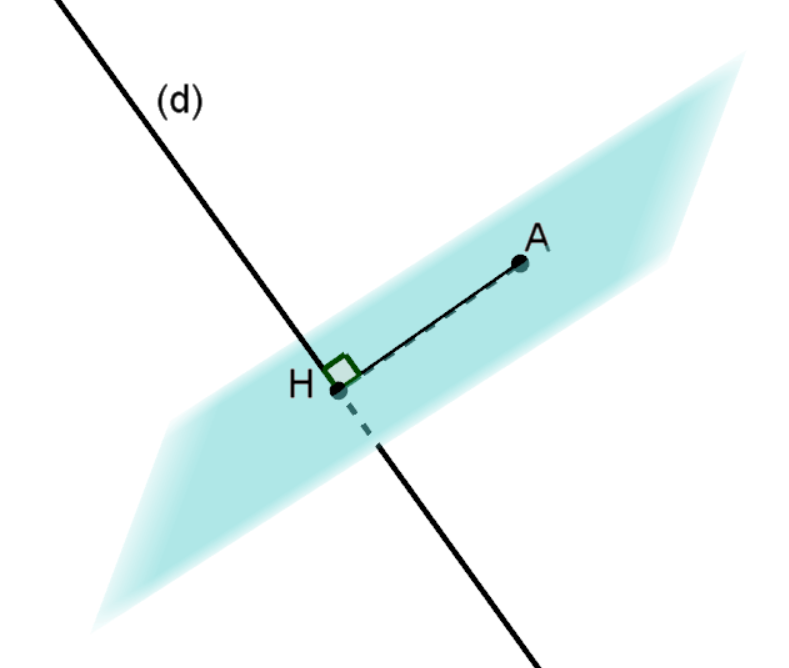
\includegraphics[scale=0.2]{projort} 
\end{center}
\end{minipage}}\hfill \fbox{\begin{minipage}{0.48\linewidth}
Projeté orthogonal de $A$ sur le plan $(P)$ : intersection du plan $(P)$ et de la droite passant par $A$ et orthogonale à $(P)$.
\begin{center}
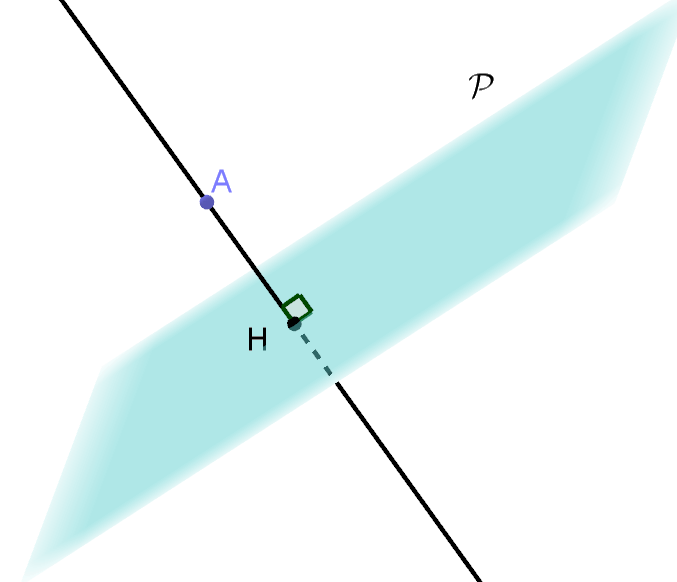
\includegraphics[scale=0.23]{projort2}
\end{center}

\end{minipage}}


\hl{\textbf{Distance}} d'un point à une droite (ou un plan) = distance du point à son projeté orthogonal

\subsection*{Équation cartésienne de plan}
\vspace{-0.5cm}
Passant par $A(x_A, y_A, z_A)$ de vecteur normal $\vec n \begin{pmatrix}a\\b\\c\end{pmatrix}$: $a(x-x_A)+b(y-y_A)+c(z-z_A)=0$

\textbf{Applications :}
\begin{itemize}
\item Déterminer directement un vecteur normal à un plan
\item Vérifier si un point appartient au plan : remplacer $x$, $y$ et $z$ par les coordonnées du point, vérifier si l'égalité est juste.
\end{itemize}

\textbf{Intersection d'une droite et d'un plan}
\begin{itemize}
\item Établir une représentation paramétrique de la droite
\item remplacer $x$, $y$ et $z$ dans l'équation du plan par ceux de la représentation paramétrique
\item trouver le paramètre $t$ en résolvant l'équation
\item remplacer ce paramètre dans la représentation de la droite.
\end{itemize}

\subsection*{Algorithmique}

\hl{\textbf{Manipulation de listes}} ; \textbf{Attention} : les indices des éléments d'une liste commencent à 0.

\begin{lstlisting}[language=python]
L1 = [] # liste vide stockee dans L1
L2 = [1, 3, 7, 6]

a = L2[0] # element d'indice 0 de L2
b = L2[1] # element d'indice 1 de L2
c = L2[-1] # dernier element de L2

c = len(L) # nombre d'elements de L2

L2.append(8) # ajoute 8 a la fin de la liste L2
L2.remove(3) #retire la premiere apparition de 3 de la liste L2
\end{lstlisting}

\textbf{Génération par compréhension}

\begin{lstlisting}[language=python]
[expression for objet in liste if condition]
\end{lstlisting}

\textbf{Itération et parcours}

\begin{lstlisting}[language = python]
range(a,b,pas) # "liste" de tous les entiers de a inclus a b exclus en progressant d'un pas donne

for i in range(n): # pour i allant de 0 a n-1
	... # indenter la partie a repeter
	
for i in L : # si L est une liste, parcourt les elements de L dans l'ordre
	... # indenter la partie a repeter
\end{lstlisting}
\end{document}